\section{High Level Synthesis in CLAS12 Trigger System Development}
\label{sec:hls}

A significant portion of the Trigger System components were developed using Vivado High-Level Synthesis (HLS) from Xilinx \cite{hls-ref}. HLS was introduced to reduce the electronics knowledge required to design hardware. It also makes the hardware design flow easier when it comes to achieving a certain behavioral model required by the hardware without worrying too much about the electronics underneath.

\subsection{Motivation to use HLS}

HLS makes it easier to incorporate well-established data processing algorithms, typically written in C++ or other high-level languages, into FPGA-based projects. HLS allows for scientists to be involved in the CLAS12 Trigger System development who do not have an electronics engineering background. It allows for the involvement of programmers who developed the algorithms for offline data processing but who have limited or no FPGA programming experience. It also makes it possible to validate code with the offline processing framework.

\subsection{Trigger Components Implemented with HLS}

HLS was used to develop most of the Stage 1 components of the CLAS12 trigger. These include the following elements:

\begin{itemize}
	\item High Threshold Cherenkov Counter (cluster energy reconstruction);
	\item Forward and Central Time-of-Flight Counters (clustering and timing correction);
	\item Electromagnetic and Preshower Calorimeters (cluster energy and position reconstruction).
\end{itemize}

The Time-of-Flight System and Cherenkov counter trigger implementation was rather straightforward. This typically takes less than 10-15\% of the Virtex-7 chip and the timing requirements were easily met.

The calorimeter trigger implementation required much more effort because of its complex nature that requires significant FPGA resources. The details are further explained in the next section using the ECAL as an example.

It should be mentioned that it took a significant amount of time to implement the desired ECAL algorithm, mostly because of the lack of experience in HLS usage. As soon as all important details of the HLS tool were understood, the development process converged, and the trigger components related to various other CLAS12 detectors were implemented in a prompt manner.


\subsection{CLAS12 Electromagnetic Calorimeters (ECAL)}

Among all of the Trigger System elements, the most challenging for the FPGA implementation was the trigger component serving the two CLAS12 electromagnetic calorimeters. Due to their structure, these calorimeters do not provide cluster coordinates or energies without significant event reconstruction. The trigger implementation details are described in Section \ref{sec:ECAL}. Below we describe our experience with HLS using ECAL as an example.


\subsection{C++ vs. HLS C++}

The FPGA implementation of the ECAL trigger was done in a 125~MHz domain, a balance between speed and resource utilization. The Trigger System components, in general, require a fixed latency, which sets certain constraints on the design. The reconstruction algorithm borrowed from the offline analysis framework was adopted for VIVADO HLS by rewriting it to C++, using HLS streams, HLS pragmas, unrolling for-loops, pipelining, and making all other needed changes. The resulting implementation was tested on simulated data and showed correct results. After that we started to run it through VIVADO HLS and VIVADO tools to address various issues related to generating an FPGA image that met the timing requirements and fit within the resource allotment.


\subsection{HLS and HDL}

When HLS is used, compiling the design consists of the following main steps:

\begin{itemize}
	\item VIVADO HLS - convert C++ to Hardware Description Language (HDL);
	\item VIVADO synthesis - HDL to FPGA primitives;
	\item VIVADO implementation - map FPGA primitives to chip and route connections.
\end{itemize}

For large designs, VIVADO HLS will very often report extremely optimistic results that suggest a viable solution, but during VIVADO implementation will fail to meet the timing requirements. To address this the failing paths must be traced back to the HLS component where it can be changed to try to improve the design. It often took many iterations to either find the workable HLS settings, code structure, or clock period adjustment.

\subsection{HLS Clock Domain}

For the different trigger components related to the different CLAS12 detectors, we use different clock domains between 250~MHz and 31.25~MHz. In the 250~MHz domain, the modules occupying more than 10\% of a XC7V550 Xilinx FPGA failed to meet the timing requirements. In the 125~MHz and lower frequency domains, the FPGA utilization was close to 100\%. For the ECAL project with a chip utilization of about 70\%, the 125~MHz clock was used.

In general, a slower clock speed (31.25~MHz) was preferable for smaller projects where resources were plentiful. When using a slow clock, the HLS code was able to be written as a single module and had no problem meeting the timing requirements during implementation.

Larger projects, such as for the ECAL, require more efficient use of the FPGA resources and have latency requirements that require a faster clock, but cannot be too fast such that the HLS modules cannot reliably meet the timing requirements. The 125~MHz clock was found to be the optimal middle ground for the ``-1'' speed grade Virtex-7 used in the CLAS12 Trigger System.


\subsection{HLS Project Size and Organization}

The typical HLS project for the CLAS12 Trigger System contains only a few routines, and uses HLS streams in the function parameter list to communicate easily with the surrounding HDL. That scheme works well for small projects.

For the ECAL with some versions being close to 100\% of FPGA utilization, the situation was quite different.
The biggest problem we faced was the inability to meet the timing requirements during the implementation (even when HLS reports that the timing is good). HLS uses state machines to schedule the operations it synthesizes. For large HLS components, the generated state machines can have massive control signal fanouts. As the clock period shrinks, so must the maximum signal fanout for the general control signals for a design to reliably meet the timing requirements. For a clock period of 8~ns using a ``-1'' speed grade Virtex-7, each HLS module was kept smaller than the 30k look-up tables (LUTs) ($<$10\% of the LUT resources) to achieve a design that consistently meets the timing requirements.

The original ECAL project consisted of about 20 C++ procedures that occupied most of the FPGA resources - with HLS generating big fanouts on this scale, it was impossible to meet the 8~ns timing on the implementation stage. The workaround was to split the entire project into smaller procedures, glued together in HDL by using well defined, simple interfaces between the separate procedures. Still, some procedures were too big, especially for the sorting algorithms. We were able to split some procedures further until finally the entire project met the timing requirements and the resulting FPGA image was loaded into the hardware.

After every significant change, we re-tested the code on simulated data, making sure it still produced correct results. The chart in Fig. ~\ref{fig:hls_chart} shows how many HLS projects were created in the end.

Another reason for subdividing the project is the lack of multi-clock domain support. Since the Event Builder in the VTP board works on a 250~MHz domain and most projects use a slower clock, every project was subdivided and separate pieces communicated over the HDL-written interface. The necessity of subdividing HLS projects and of using HDL to assemble them together, is probably the most restricting feature in HLS usage. Much of this subdividing can be reduced by using the HLS DATAFLOW directives (which can isolate functions communicating through registered FIFO interfaces), but it requires further code restructuring to be compatible with this flow and does not support multiple clock domains.

\begin{figure}[hbt]
	\centering
	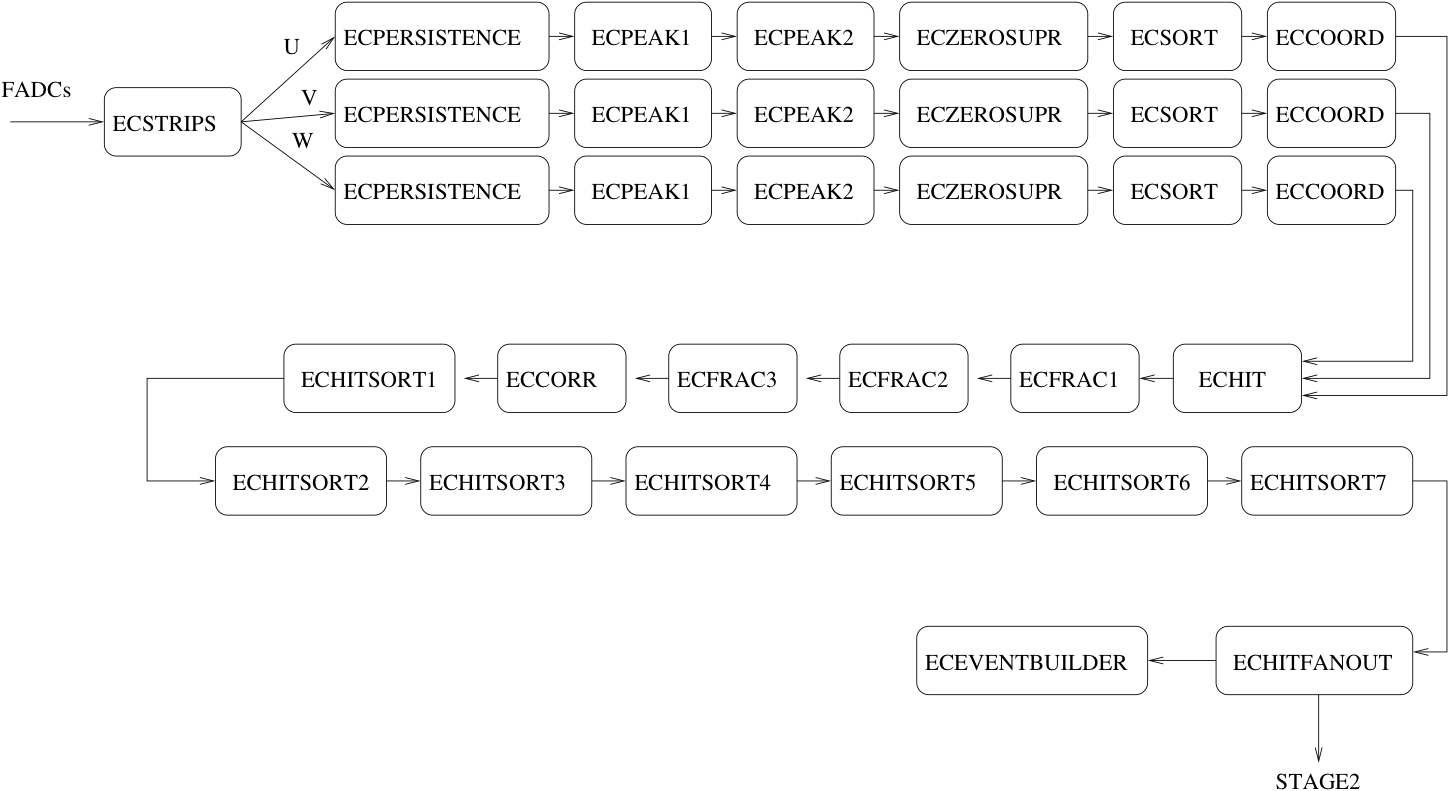
\includegraphics[width=1.0\columnwidth,keepaspectratio]{img/hls_chart.png}
	\caption{ECAL HLS project chart. The entire project is split into multiple smaller projects to satisfy the timing requirements. In particular, the hit sorting section is split into seven identical projects.}
	\label{fig:hls_chart}
\end{figure}


\subsection{HLS Versions and Cross-Project Dependences}

As mentioned before, splitting the project into smaller pieces allowed us to meet the timing requirements. This worked, in particular, because we were able to eliminate combinatorial paths between the HLS projects connected by the streams. Such dependences can be clearly seen looking into the schematics for the failed timing chains, and were usually related to the large state machine control signals going between modules. Initially we used HLS version 2015, and despite all of our efforts, we could not eliminate these long combinatorial paths across modules. This was resolved after switching to HLS version 2017, where the streams could be fully registered (with pragma ``axis register both port=''). This meant that if the registered HLS streams were used between separate HLS projects, then the state machine paths were also registered between modules. With that, it was only a matter of splitting projects into smaller pieces to improve/meet the timing requirements.


\subsection{HLS Settings}

The clock uncertainty is set as 30\% of the main clock, which we found forces HLS to produce more realistic timing estimates. A single HLS project often cannot exceed several percent of the flip-flops (FF) and LUT budget, otherwise it may be a problem to meet the timing requirement on the VIVADO implementation step. A typical HLS project for one of the PCAL trigger elements is shown in Fig. ~\ref{fig:hls}.

\begin{figure}[hbt]
	\centering
	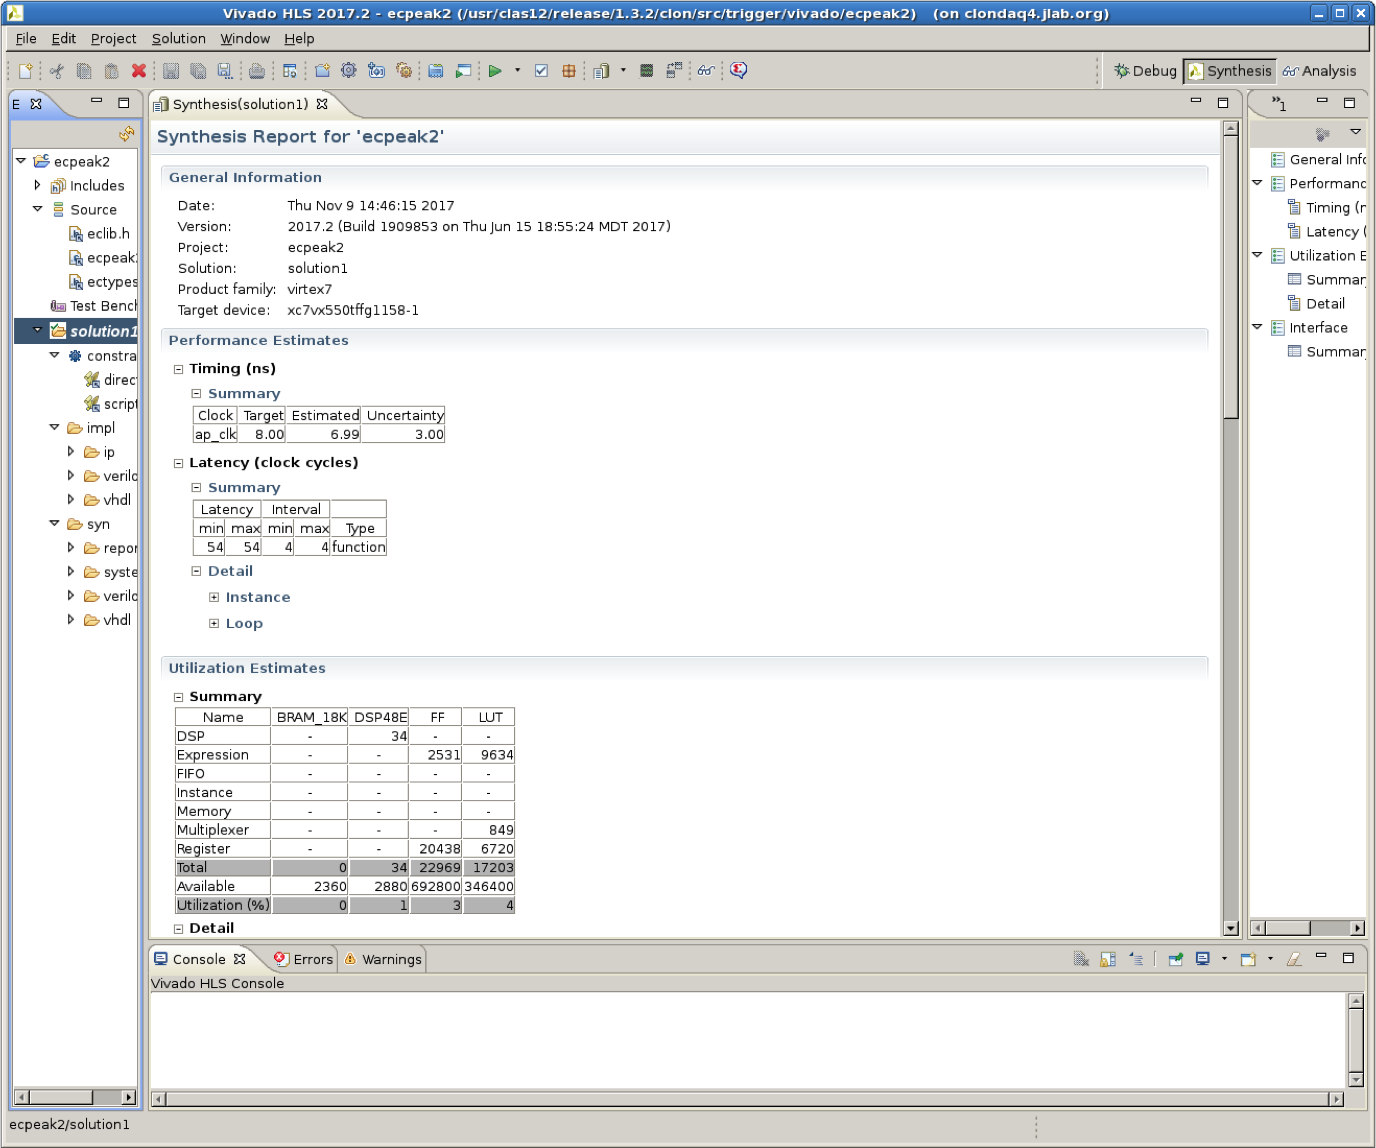
\includegraphics[width=1.0\columnwidth,keepaspectratio]{img/hls.png}
	\caption{Typical HLS project for one of the PCAL trigger elements. 4\% LUTs is close to the maximum possible to meet the timing requirements of the following steps. With an 8~ns target, the clock uncertainty  is set to 3~ns.}
	\label{fig:hls}
\end{figure}

\subsection{VIVADO Settings}

Common settings for VIVADO were used as shown in Fig. ~\ref{fig:vivado}. It usually takes 3+ hours to compile the PCAL project on a Dell R730 server under RHEL7. For some firmware versions, we were able to utilize 100\% of the LUTs and still meet the timing requirements if the clock domain was 125~MHz or lower. The VIVADO project for the PCAL trigger is shown in Fig. ~\ref{fig:vivado}.

\begin{figure}[hbt]
	\centering
	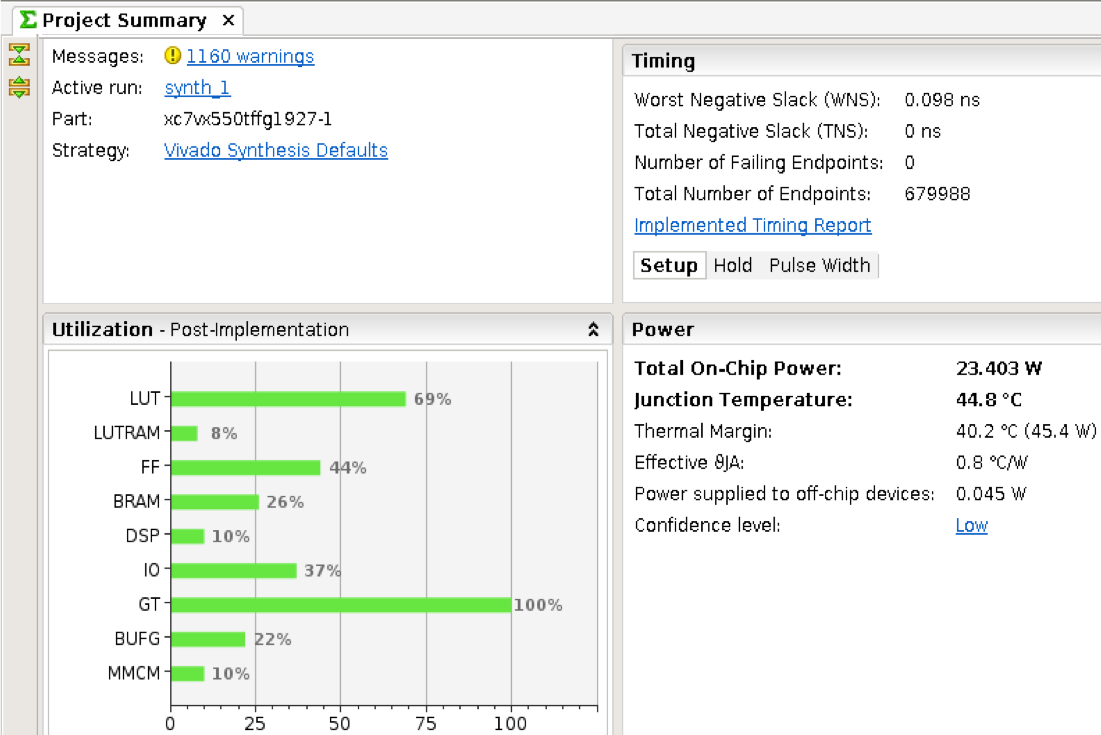
\includegraphics[width=1.0\columnwidth,keepaspectratio]{img/vivado.png}
	\caption{VIVADO project for the PCAL trigger. Strategies used were ``Vivado Synthesis Defaults'' and ``Performance\_ExplorePostRoutePhysOpt''. LUT utilization is about 2/3 of the total balance. It was relatively easy to meet the timing requirements with an FPGA clock 125~MHz or slower.}
	\label{fig:vivado}
\end{figure}

\subsection{Firmware Validation for HLS-based Projects}

The ability to validate the firmware using a C++ implementation is the one of the biggest advantages of HLS. During the course of development and commissioning, we ran HLS C++ code on simulated and real data from the CLAS12 detectors, implementing required features and fixing bugs. During data taking we were able to find and fix observed problems or add new features in several hours, which was very important to save beam time.

\subsection{Our Conclusion about HLS Usage}

The CLAS12 ECAL and other detectors were successfully implemented into the Trigger System using HLS to produce the core part of the firmware. This trigger was used in the first physics run in 2018 and worked as expected. We were able to select events based on individual ECAL cluster energy, something which was possible before only during offline data processing.

HLS in general appears to be a useful tool, especially to implement smaller trigger components like the Cherenkov or Time-of-Flight counters. For components utilizing a significant portion of the FPGA, it will benefit development significantly to improve HLS in the following directions:

\begin{itemize}
	\item Support multi-clock domains;
	\item Improve subroutine calls by allowing the option to fully register paths between modules; 
	\item Improve state machine logic, for example support streams between routines inside the project and be able to generate separate state machines for separate routines. This will allow for the avoidance of splitting the project manually and using HDL as a top interface as we are currently forced to do.
\end{itemize}
